\documentclass[11pt,a4paper,]{article}
\usepackage{lmodern}

\usepackage{amssymb,amsmath}
\usepackage{ifxetex,ifluatex}
\usepackage{fixltx2e} % provides \textsubscript
\ifnum 0\ifxetex 1\fi\ifluatex 1\fi=0 % if pdftex
  \usepackage[T1]{fontenc}
  \usepackage[utf8]{inputenc}
\else % if luatex or xelatex
  \usepackage{unicode-math}
  \defaultfontfeatures{Ligatures=TeX,Scale=MatchLowercase}
\fi
% use upquote if available, for straight quotes in verbatim environments
\IfFileExists{upquote.sty}{\usepackage{upquote}}{}
% use microtype if available
\IfFileExists{microtype.sty}{%
\usepackage[]{microtype}
\UseMicrotypeSet[protrusion]{basicmath} % disable protrusion for tt fonts
}{}
\PassOptionsToPackage{hyphens}{url} % url is loaded by hyperref
\usepackage[unicode=true]{hyperref}
\hypersetup{
            pdftitle={Analysis of World Alcohol Consumption},
            pdfborder={0 0 0},
            breaklinks=true}
\urlstyle{same}  % don't use monospace font for urls
\usepackage{geometry}
\geometry{a4paper, centering, text={16cm,25cm}}
\usepackage[style=authoryear-comp,]{biblatex}
\addbibresource{references.bib}
\usepackage{longtable,booktabs}
% Fix footnotes in tables (requires footnote package)
\IfFileExists{footnote.sty}{\usepackage{footnote}\makesavenoteenv{long table}}{}
\IfFileExists{parskip.sty}{%
\usepackage{parskip}
}{% else
\setlength{\parindent}{0pt}
\setlength{\parskip}{6pt plus 2pt minus 1pt}
}
\setlength{\emergencystretch}{3em}  % prevent overfull lines
\providecommand{\tightlist}{%
  \setlength{\itemsep}{0pt}\setlength{\parskip}{0pt}}
\setcounter{secnumdepth}{5}

% set default figure placement to htbp
\makeatletter
\def\fps@figure{htbp}
\makeatother


\title{Analysis of World Alcohol Consumption}

%% MONASH STUFF

%% CAPTIONS
\RequirePackage{caption}
\DeclareCaptionStyle{italic}[justification=centering]
 {labelfont={bf},textfont={it},labelsep=colon}
\captionsetup[figure]{style=italic,format=hang,singlelinecheck=true}
\captionsetup[table]{style=italic,format=hang,singlelinecheck=true}


%% FONT
\RequirePackage{bera}
\RequirePackage[charter,expert,sfscaled]{mathdesign}
\RequirePackage{fontawesome}

%% HEADERS AND FOOTERS
\RequirePackage{fancyhdr}
\pagestyle{fancy}
\rfoot{\Large\sffamily\raisebox{-0.1cm}{\textbf{\thepage}}}
\makeatletter
\lhead{\textsf{\expandafter{\@title}}}
\makeatother
\rhead{}
\cfoot{}
\setlength{\headheight}{15pt}
\renewcommand{\headrulewidth}{0.4pt}
\renewcommand{\footrulewidth}{0.4pt}
\fancypagestyle{plain}{%
\fancyhf{} % clear all header and footer fields
\fancyfoot[C]{\sffamily\thepage} % except the center
\renewcommand{\headrulewidth}{0pt}
\renewcommand{\footrulewidth}{0pt}}

%% MATHS
\RequirePackage{bm,amsmath}
\allowdisplaybreaks

%% GRAPHICS
\RequirePackage{graphicx}
\setcounter{topnumber}{2}
\setcounter{bottomnumber}{2}
\setcounter{totalnumber}{4}
\renewcommand{\topfraction}{0.85}
\renewcommand{\bottomfraction}{0.85}
\renewcommand{\textfraction}{0.15}
\renewcommand{\floatpagefraction}{0.8}


%\RequirePackage[section]{placeins}

%% SECTION TITLES


%% SECTION TITLES
\RequirePackage[compact,sf,bf]{titlesec}
\titleformat*{\section}{\Large\sf\bfseries\color[rgb]{0.7,0,0}}
\titleformat*{\subsection}{\large\sf\bfseries\color[rgb]{0.7,0,0}}
\titleformat*{\subsubsection}{\sf\bfseries\color[rgb]{0.7,0,0}}
\titlespacing{\section}{0pt}{2ex}{.5ex}
\titlespacing{\subsection}{0pt}{1.5ex}{0ex}
\titlespacing{\subsubsection}{0pt}{.5ex}{0ex}


%% TITLE PAGE
\def\Date{\number\day}
\def\Month{\ifcase\month\or
 January\or February\or March\or April\or May\or June\or
 July\or August\or September\or October\or November\or December\fi}
\def\Year{\number\year}

%% LINE AND PAGE BREAKING
\sloppy
\clubpenalty = 10000
\widowpenalty = 10000
\brokenpenalty = 10000
\RequirePackage{microtype}

%% PARAGRAPH BREAKS
\setlength{\parskip}{1.4ex}
\setlength{\parindent}{0em}

%% HYPERLINKS
\RequirePackage{xcolor} % Needed for links
\definecolor{darkblue}{rgb}{0,0,.6}
\RequirePackage{url}

\makeatletter
\@ifpackageloaded{hyperref}{}{\RequirePackage{hyperref}}
\makeatother
\hypersetup{
     citecolor=0 0 0,
     breaklinks=true,
     bookmarksopen=true,
     bookmarksnumbered=true,
     linkcolor=darkblue,
     urlcolor=blue,
     citecolor=darkblue,
     colorlinks=true}

\usepackage[showonlyrefs]{mathtools}
\usepackage[no-weekday]{eukdate}

%% BIBLIOGRAPHY

\makeatletter
\@ifpackageloaded{biblatex}{}{\usepackage[style=authoryear-comp, backend=biber, natbib=true]{biblatex}}
\makeatother
\ExecuteBibliographyOptions{bibencoding=utf8,minnames=1,maxnames=3, maxbibnames=99,dashed=false,terseinits=true,giveninits=true,uniquename=false,uniquelist=false,doi=false, isbn=false,url=true,sortcites=false}

\DeclareFieldFormat{url}{\texttt{\url{#1}}}
\DeclareFieldFormat[article]{pages}{#1}
\DeclareFieldFormat[inproceedings]{pages}{\lowercase{pp.}#1}
\DeclareFieldFormat[incollection]{pages}{\lowercase{pp.}#1}
\DeclareFieldFormat[article]{volume}{\mkbibbold{#1}}
\DeclareFieldFormat[article]{number}{\mkbibparens{#1}}
\DeclareFieldFormat[article]{title}{\MakeCapital{#1}}
\DeclareFieldFormat[article]{url}{}
%\DeclareFieldFormat[book]{url}{}
%\DeclareFieldFormat[inbook]{url}{}
%\DeclareFieldFormat[incollection]{url}{}
%\DeclareFieldFormat[inproceedings]{url}{}
\DeclareFieldFormat[inproceedings]{title}{#1}
\DeclareFieldFormat{shorthandwidth}{#1}
%\DeclareFieldFormat{extrayear}{}
% No dot before number of articles
\usepackage{xpatch}
\xpatchbibmacro{volume+number+eid}{\setunit*{\adddot}}{}{}{}
% Remove In: for an article.
\renewbibmacro{in:}{%
  \ifentrytype{article}{}{%
  \printtext{\bibstring{in}\intitlepunct}}}

\AtEveryBibitem{\clearfield{month}}
\AtEveryCitekey{\clearfield{month}}

\makeatletter
\DeclareDelimFormat[cbx@textcite]{nameyeardelim}{\addspace}
\makeatother

\author{\sf{\Large\textbf{Aishwarya Anil Kumar}\\\large \href{mailto:aani0005@monash.student.com}{\nolinkurl{aani0005@monash.student.com}}\\[0.5cm]}{\Large\textbf{Amrita Jena}\\\large \href{mailto:ajen0022@student.monash.edu}{\nolinkurl{ajen0022@student.monash.edu}}\\[0.5cm]}{\Large\textbf{Priyasha Saini}\\\large \href{mailto:psai0005@student.monash.edu}{\nolinkurl{psai0005@student.monash.edu}}\\[0.5cm]}{\Large\textbf{Xuan Nhat Minh Nguyen}\\\large \href{mailto:xngu0008@student.monash.edu}{\nolinkurl{xngu0008@student.monash.edu}}\\[0.5cm]}}

\date{\sf\Date~\Month~\Year}
\makeatletter
\lfoot{\sf Kumar, Jena, Saini, Nguyen: \@date}
\makeatother


%%%% PAGE STYLE FOR FRONT PAGE OF REPORTS

\makeatletter
\def\organization#1{\gdef\@organization{#1}}
\def\telephone#1{\gdef\@telephone{#1}}
\def\email#1{\gdef\@email{#1}}
\makeatother
  \organization{Monash University}

  \def\name{Department of \hbox{Econometrics \&} \hbox{Business Statistics}}

  \telephone{(03) 9905 2478}

  \email{BusEco-Econometrics@monash.edu}

\def\webaddress{\url{http://buseco.monash.edu/ebs/consulting/}}
\def\abn{12 377 614 012}
\def\extraspace{\vspace*{1.6cm}}
\makeatletter
\def\contactdetails{\faicon{phone} & \@telephone \\
                    \faicon{envelope} & \@email}
\makeatother

\usepackage[absolute,overlay]{textpos}
\setlength{\TPHorizModule}{1cm}
\setlength{\TPVertModule}{1cm}

%%%% FRONT PAGE OF REPORTS

\def\reporttype{Report for}

\long\def\front#1#2#3{
\newpage
\begin{textblock}{7}(12.7,28.2)\hfill

\includegraphics[height=0.6cm]{AACSB}~~~

\includegraphics[height=0.6cm]{EQUIS}~~~

\includegraphics[height=0.6cm]{AMBA}
\end{textblock}
\begin{singlespacing}
\thispagestyle{empty}
\vspace*{-1.4cm}
\hspace*{-1.4cm}
\hbox to 16cm{
  \hbox to 6.5cm{\vbox to 14cm{\vbox to 25cm{
    
\includegraphics[width=6cm]{monash2}
    \vfill
    
\includegraphics[width=3.5cm]{MBSportrait}
    \vspace{0.4cm}
    \par
    \parbox{6.3cm}{\raggedright
      \sf\color[rgb]{0.00,0.00,0.70}
      {\large\textbf{\name}}\par
      \vspace{.7cm}
      \tabcolsep=0.12cm\sf\small
      \begin{tabular}{@{}ll@{}}\contactdetails
      \end{tabular}
      \vspace*{0.3cm}\par
      ABN: \abn\par
    }
  }\vss}\hss}
  \hspace*{0.2cm}
  \hbox to 1cm{\vbox to 14cm{\rule{1pt}{26.8cm}\vss}\hss\hfill}
  \hbox to 10cm{\vbox to 14cm{\vbox to 25cm{
      \vspace*{3cm}\sf\raggedright
      \parbox{11cm}{\sf\raggedright\baselineskip=1.2cm
         \fontsize{24.88}{30}\color[rgb]{0.70,0.00,0.00}\sf\textbf{#1}}
      \par
      \vfill
      \large
      \vbox{\parskip=0.8cm #2}\par
      \vspace*{2cm}\par
      \reporttype\\[0.3cm]
      \hbox{#3}%\\[2cm]\
      \vspace*{1cm}
      {\large\sf\textbf{\Date~\Month~\Year}}
   }\vss}
  }}
\end{singlespacing}
\newpage
}

\makeatletter
\def\titlepage{\front{\expandafter{\@title}}{\@author}{\@organization}}
\makeatother

\usepackage{setspace}
\setstretch{1.5}

%% Any special functions or other packages can be loaded here.
\usepackage{booktabs}
\usepackage{longtable}
\usepackage{array}
\usepackage{multirow}
\usepackage{wrapfig}
\usepackage{float}
\usepackage{colortbl}
\usepackage{pdflscape}
\usepackage{tabu}
\usepackage{threeparttable}
\usepackage{threeparttablex}
\usepackage[normalem]{ulem}
\usepackage{makecell}
\usepackage{xcolor}


\begin{document}
\titlepage

{
\setcounter{tocdepth}{2}
\tableofcontents
}
\pagebreak

\section{Executive summary}\label{executive-summary}

The \textcite{owidalcoholconsumption} website contains a thorough examination of alcohol consumption trends. The statistics revealed that, with a few notable exceptions, alcohol consumption has vastly increased worldwide over time. Additionally, alcohol consumption varied greatly by nation, with some having significantly higher levels than others.

The primary objective of this report is to provide organizations with insights into this issue and encourage the establishment of strategies and policies in order to mitigate such harmful influences of excessive alcohol consumption and avert potential hazards.

The report endeavors to analyze the the prevalence of alcohol use and the most popular beverage. Moreover, it also consider the global patterns of alcohol expenditure by investigating the data of alcohol consumption versus GDP per capita and population in 2018 as well as alcohol expenditure by places in the USA. Furthermore, the mental health issues due to alcohol, also known as Alcohol Use Disorder (AUD), is mentioned by analyzing leading countries in this issue and its distribution worldwide compared to population by means of standard measures. Lastly, the global trend in road-traffic deaths due to alcohol will be analyzed to support the adverse influence of alcohol consumption.

On analyzing the data, we also come to an understanding that alcohol consumption varied greatly by nation, beer is the most popular beverage, followed by wine and spirits, the ratio of individuals suffering from AUD is much higher in some countries as compared to most other countries indicating the population in some places being more prone to alcoholism, and there is significant variation in standard alcohol drinking measures across the different countries, which can be obtained from the latest data available.

Policymakers and public health professionals can utilize these findings to help them create measures to combat the negative impacts of excessive alcohol use in their particular nations.

\pagebreak

\section{Introduction}\label{introduction}

Social drinking, around the world, has always been part of the society and enjoyed by many. Binge drinking among youth is becoming more and more popular especially as a leisure activity.
Despite its high consumption rate, alcohol exerts detrimental effects on society, such as compromising human health, causing accidents, and leading to social problems. According to \textcite{nationalnational}, Alcohol Use Disorder(AUD) is one such risk factor which mainly refers to mental health problems caused due to heavy alcohol consumption. This can cause a negative concussion on social and economic conditions. Furthermore, it burdens people with financial constraints like hampering their income. As a result, this controversial issue has attracted concerns from many researchers and policymakers who desire to improve the current situation and stabilize society.

The figure \ref{fig:worldmap} shows the total alcohol that has been consumed per person for the year 2018. The above image has been taken from the \textcite{owidalcoholconsumption} website.

\begin{figure}

{\centering 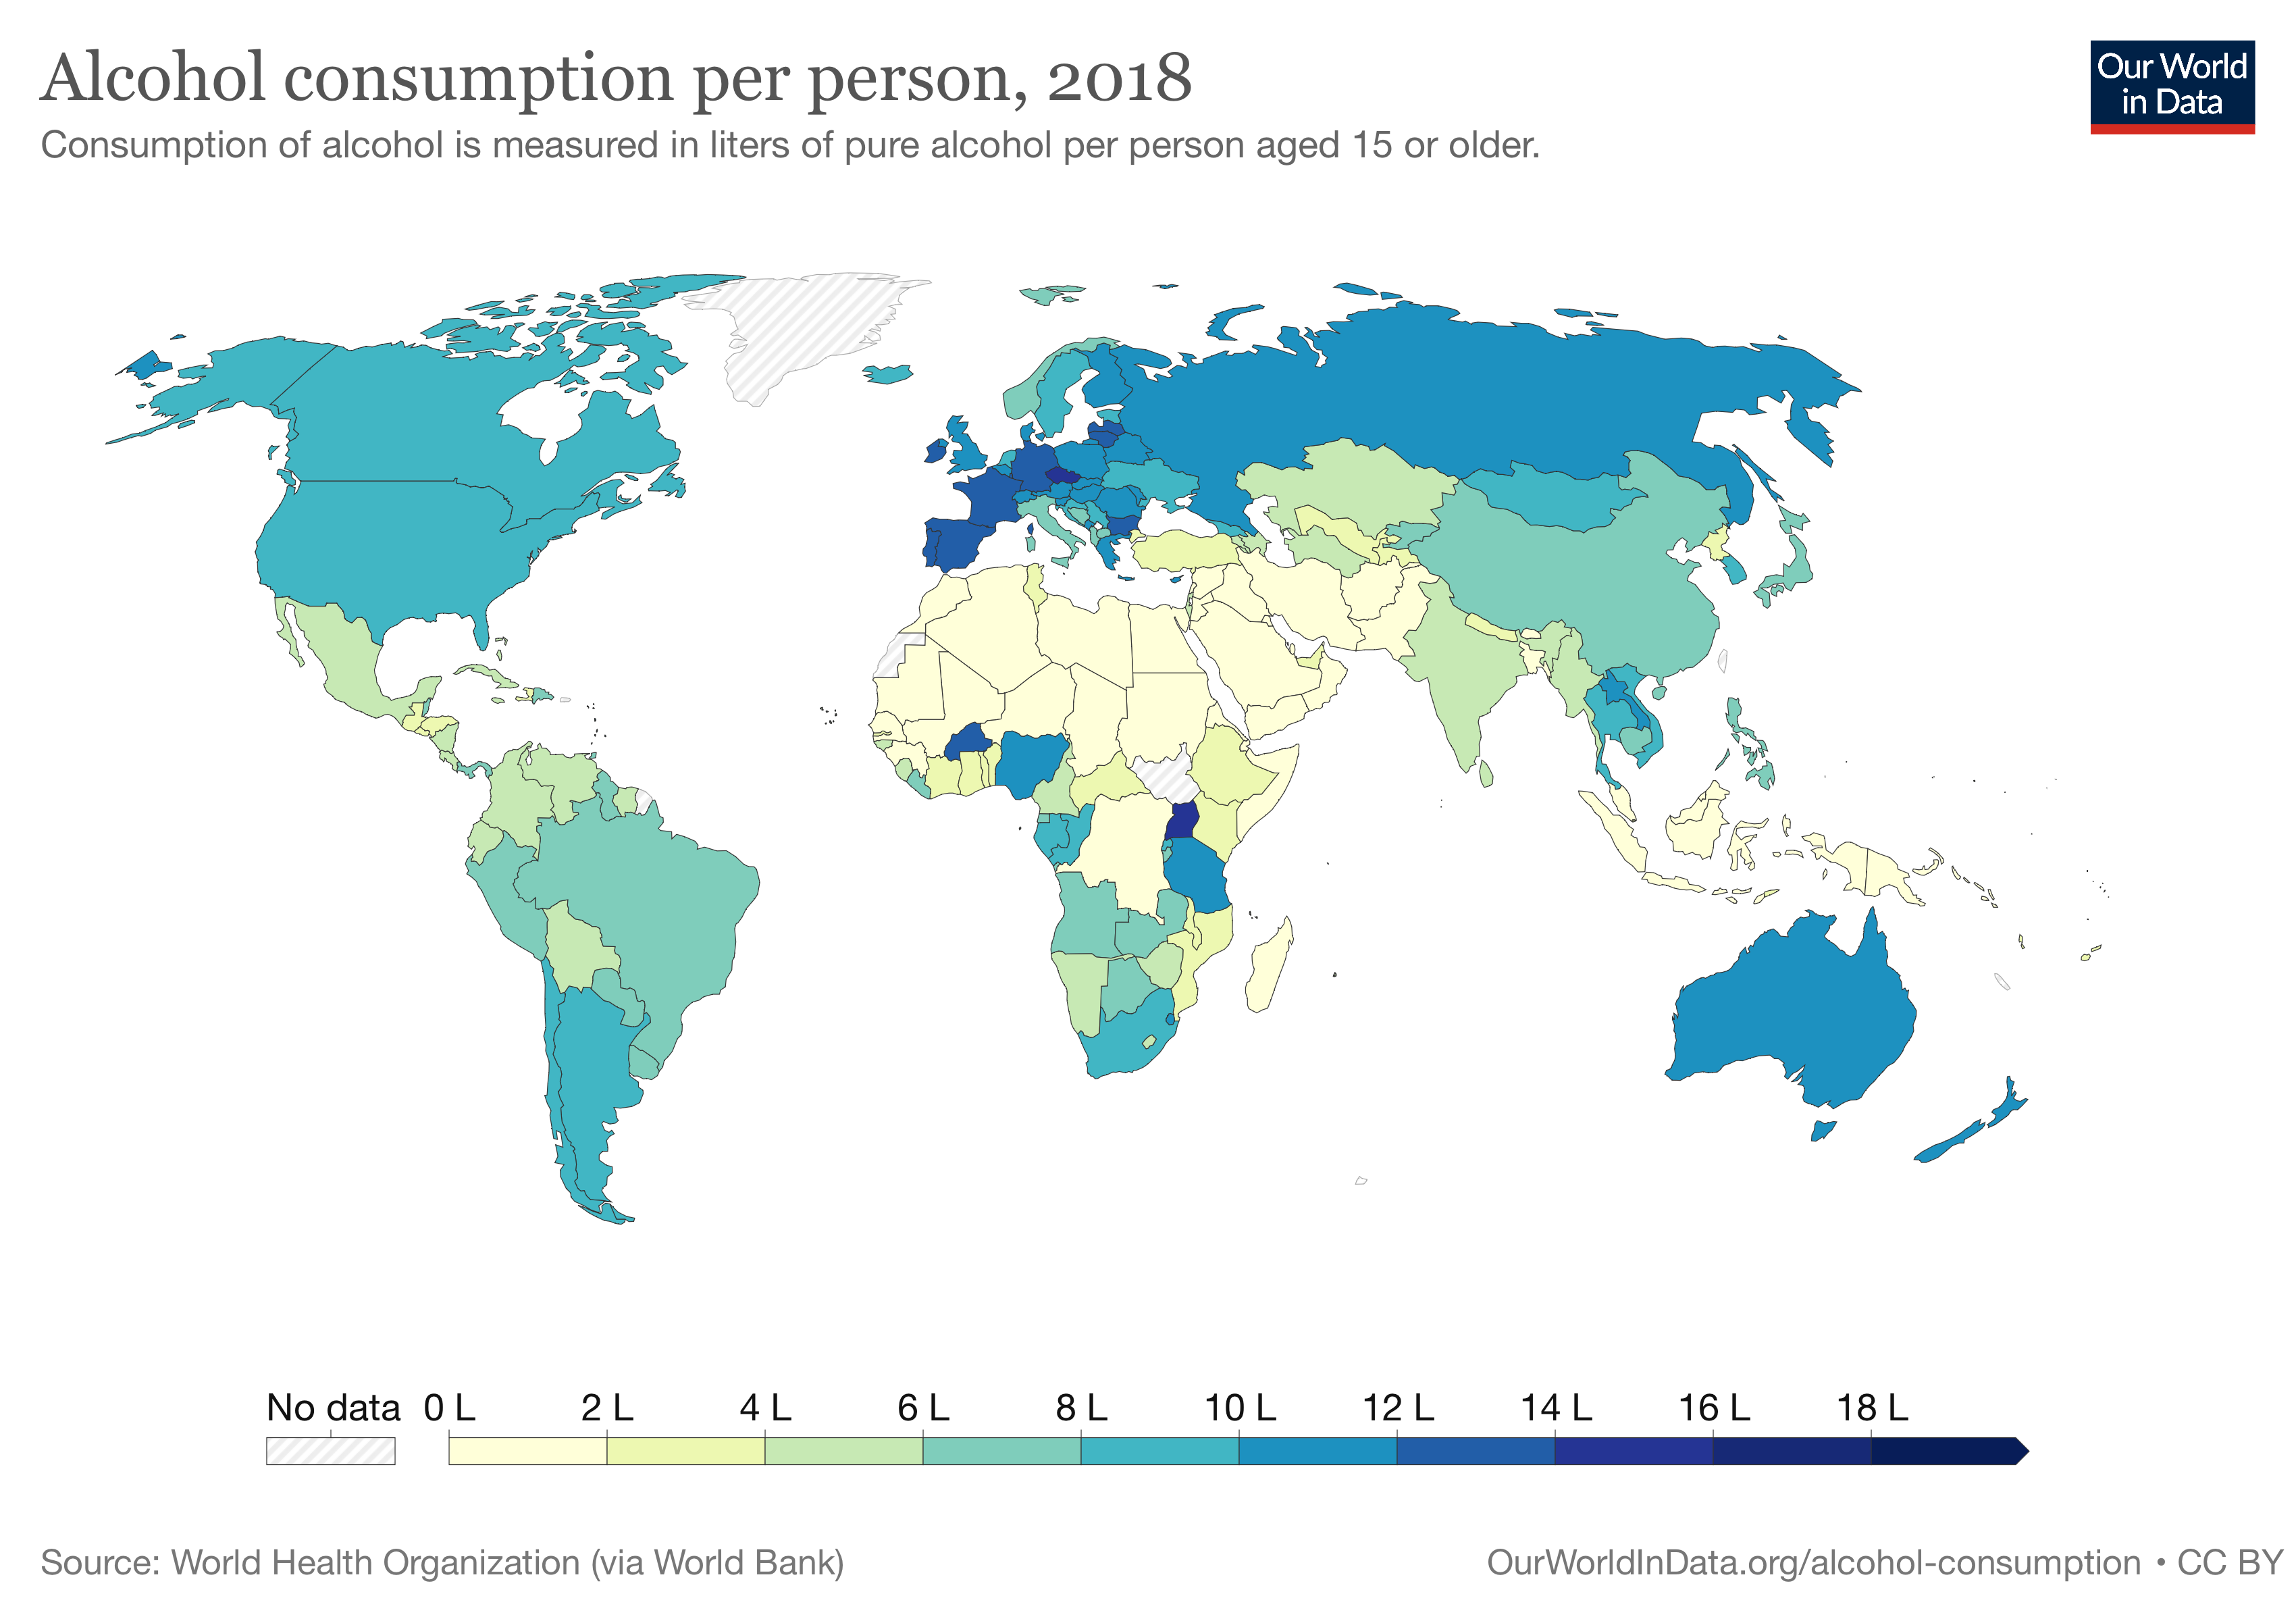
\includegraphics[width=400px,height=250px]{images/worldmap} 

}

\caption{Alcohol consumption per person for the world for 2018}\label{fig:worldmap}
\end{figure}

With the supporting data from \href{https://ourworldindata.org/}{Our world in data}, this report will summarize
- overall alcohol intake, types of beverages consumed across the globe and has the beverage preference changed over the years, if yes, which countries has the most number of consumers based on the beverage types.
- the disparities in alcohol expenditure will also be examined by analyzing its relationship with GDP per capita and population. This was conducted to provide insights into our doubts about whether wealthier or more populated countries consume more alcohol than the others.
- the conditions such as alcohol abuse or alcohol addiction(AUD) can be different in different people ranging from mild, moderate, or severe. Hence, recognizing pattern and proper diagnosis can be helpful.
- impact of alcohol consumption on road safety, as it is one of the major causes of road accident deaths worldwide. It has also been found that there exists a correlation between the amount of alcohol consumed and people involved in road traffic accidents.

\section{Methodology}\label{methodology}

This report's technical analysis uses the following R packages: \newline
- tidyverse by \textcite{tidyverse} \newline
- ggplot2 by \textcite{ggplot2} \newline
- bookdown by \textcite{Xie2020-es} \newline
- tinytex by \textcite{tinytex} \newline
- kableExtra by \textcite{kableExtra} \newline
- broom by \textcite{broom} \newline
- here by \textcite{here} \newline
- ggrepel by \textcite{ggrepel} \newline
- knitr by \textcite{knitr} \newline
- rmarkdown by \textcite{rmarkdown} \newline

\subsection{Alcohol Beverage preferences across the globe}\label{alcohol-beverage-preferences-across-the-globe}

Although the word ``alcohol'' has been used extensively, it actually refers to a variety of drinks. Beer, Spirits, and Wine are the solution portion to it which can be seen in figure \ref{fig:beveragestype}. Comparing the data for the earliest and most recent year available will provide you the classification of alcohol and any significant shifts in patterns of its usage that are relevant to the circumstances at hand.
The data has been taken from \textcite{owidalcoholconsumption}

\begin{figure}

{\centering 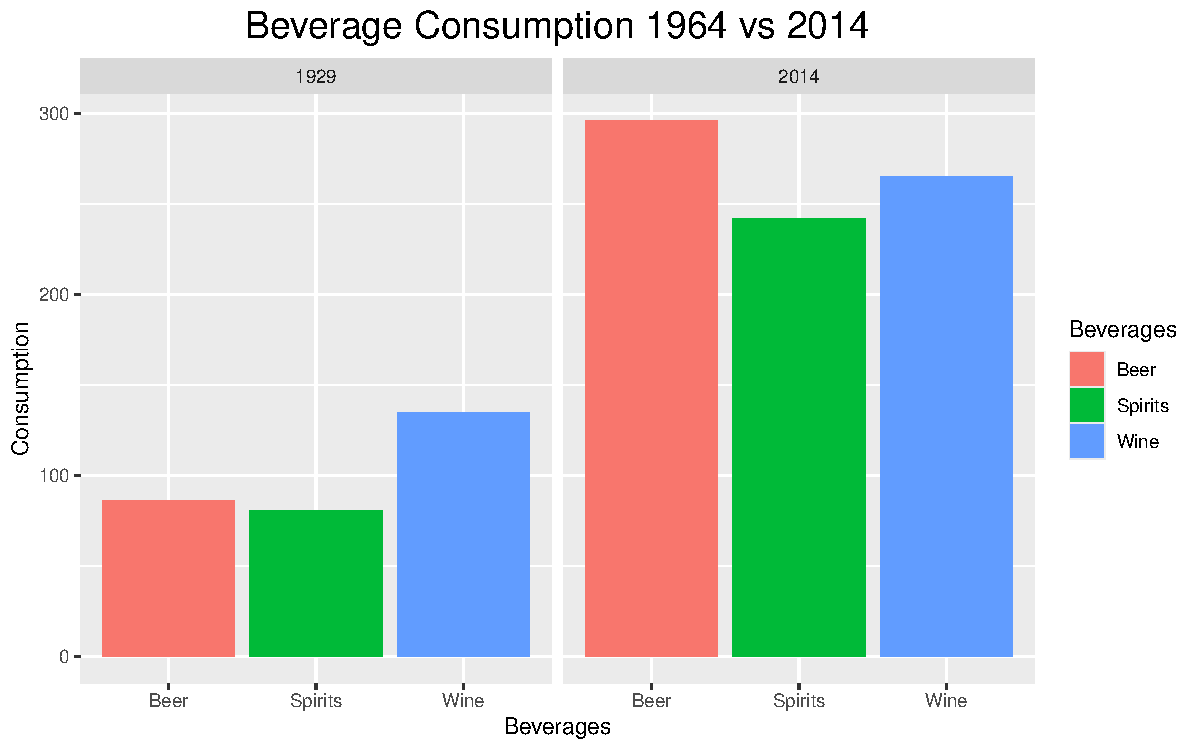
\includegraphics[width=400px,height=250px]{alcohol_analysis_files/figure-latex/beveragestype-1} 

}

\caption{Beverage Consumption 1964 vs 2014}\label{fig:beveragestype}
\end{figure}

Based on the consumption of each beverage, the table \ref{tab:table} displays a relationship between the most preferred beverage type. This is accomplished by computing the maximum values among beer, wine, and spirits and then determining which sort of alcohol is most preferred one.

\begin{table}

\caption{\label{tab:table}Preferred Beverage in Different Countries}
\centering
\begin{tabular}[t]{c|c|c}
\hline
Country & Max\_alcohol & Alcohol\_Type\\
\hline
Australia & 46 & Beer\\
\hline
Austria & 51 & Beer\\
\hline
Belgium & 51 & Beer\\
\hline
Canada & 49 & Beer\\
\hline
Denmark & 47 & Wine\\
\hline
Finland & 53 & Beer\\
\hline
France & 59 & Wine\\
\hline
Italy & 65 & Wine\\
\hline
Japan & 74 & Spirits\\
\hline
Netherlands & 48 & Beer\\
\hline
New Zealand & 43 & Beer\\
\hline
Norway & 36 & Spirits\\
\hline
Sweden & 48 & Wine\\
\hline
Switzerland & 47 & Wine\\
\hline
United Kingdom & 41 & Wine\\
\hline
United States & 49 & Beer\\
\hline
\end{tabular}
\end{table}
\pagebreak

\subsection{Alcohol's impact on finances: Exploring the relationship between income and expenditure}\label{alcohols-impact-on-finances-exploring-the-relationship-between-income-and-expenditure}

In order to fulfill our aim, a precise analysis of worldwide alcohol expenditure is performed based on reliable information obtained from the \href{https://ourworldindata.org/alcohol-consumption}{Alcohol Consumption} article on the \href{https://ourworldindata.org/}{Our world in data} website.

To analyze the expenditure on alcohol, two data sets are used to provide more insights. The first data set contains the world's alcohol consumption, GDP per capita, and population in 2018 by countries and continents which is the most recently available data.
Figure \ref{fig:GDP-vs-Consumption} and figure \ref{fig:Population-vs-Consumption} show the relationship between alcohol consumption with income and population. Both figures provide some insights into whether linear relationships exist between alcohol consumption (liters per capita) and either GDP per capita or population in 2018. The second data set contains the alcohol expenditure by places in the USA from 1997 to 2021.

\begin{figure}

{\centering 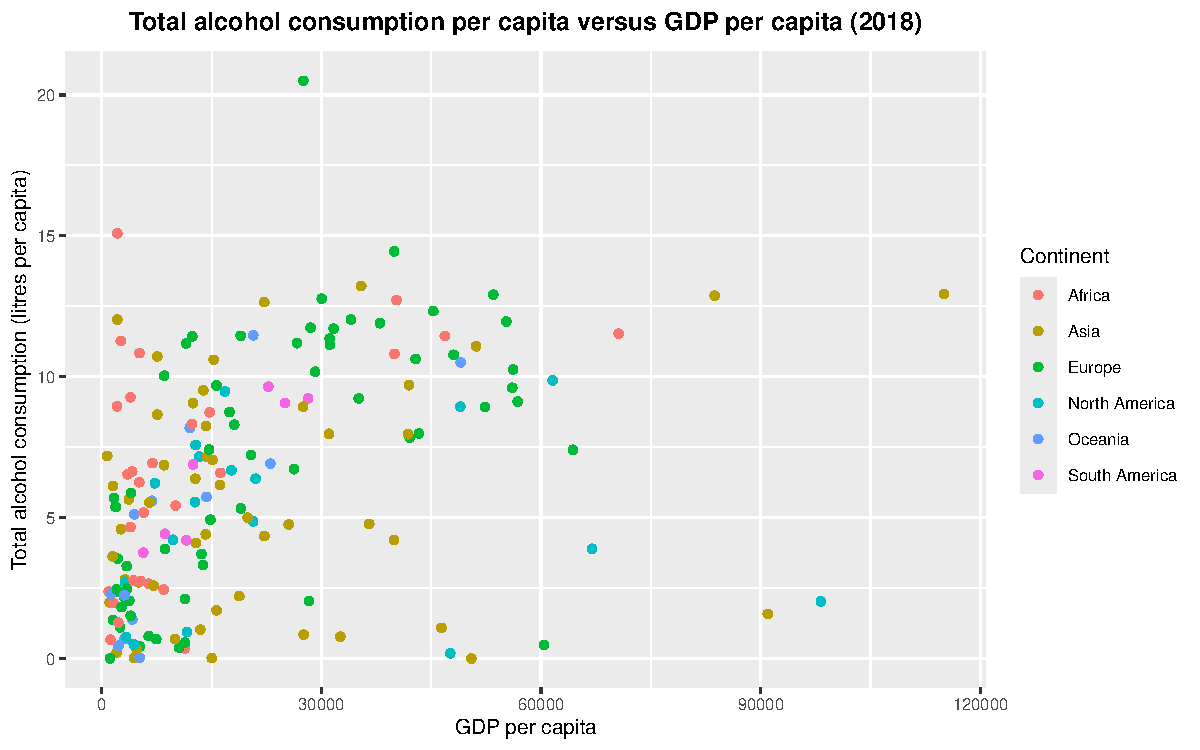
\includegraphics[width=0.7\linewidth]{alcohol_analysis_files/figure-latex/GDP-vs-Consumption-1} 

}

\caption{Scatterplot between the Alcohol Consumption versus GDP per capita in 2018 among continents.}\label{fig:GDP-vs-Consumption}
\end{figure}
\begin{figure}

{\centering 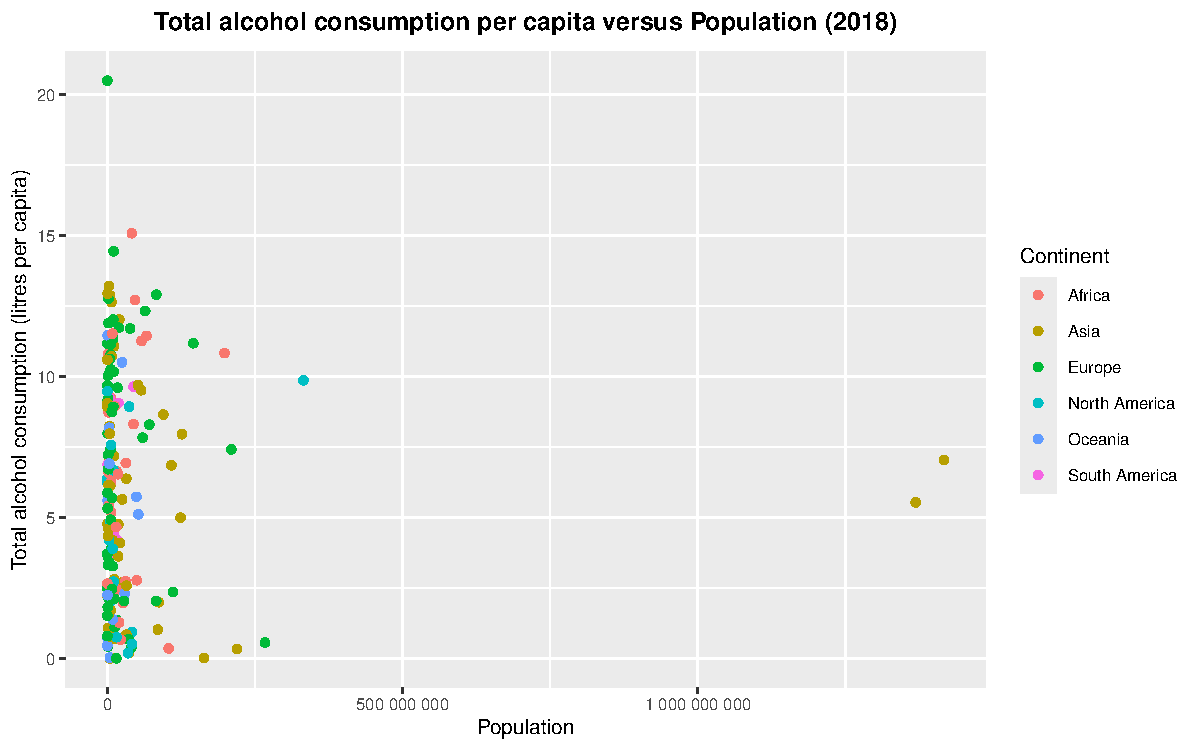
\includegraphics[width=0.7\linewidth]{alcohol_analysis_files/figure-latex/Population-vs-Consumption-1} 

}

\caption{Scatterplot between the Alcohol Consumption versus Population in 2018 among continents.}\label{fig:Population-vs-Consumption}
\end{figure}

Besides scatterplots, linear regression models can also effectively assist in analyzing these relationships. table \ref{tab:lm-gdp-cons} and table \ref{tab:lm-pop-cons} show the statistical summary of linear regression models of total alcohol consumption per capita versus GDP per capita and population in 2018 respectively. The efficiency of both linear regression models can be measured by the reported \(R^2\) and \(p-value\) from the summary of models. The \(R^2\) explains the percentage of changes in the dependent variable being explained by changes in the independent variable. A high \(R^2\) indicates the possibility of the model fitting data well. The \(p-value\) supports the evidence of variables being statistically significant for predicting dependent variable. If the \(p-value\) is greater than 0.5, there is insufficient evidence that the variable is statistically significant at 95\% significance level.

\begin{table}

\caption{\label{tab:lm-gdp-cons}Statistic summary of linear regression model between Total alcohol consumption per capita and GDP per capita in 2018}
\centering
\begin{tabular}[t]{l|r|r|r|r}
\hline
term & estimate & std.error & statistic & p.value\\
\hline
(Intercept) & 4.5276065 & 0.4015177 & 11.276231 & 0e+00\\
\hline
`GDP per capita` & 0.0000773 & 0.0000140 & 5.540688 & 1e-07\\
\hline
\end{tabular}
\end{table}
\begin{table}

\caption{\label{tab:lm-pop-cons}Statistic summary of linear regression model between Total alcohol consumption per capita and Population in 2018}
\centering
\begin{tabular}[t]{l|r|r|r|r}
\hline
term & estimate & std.error & statistic & p.value\\
\hline
(Intercept) & 6.091135 & 0.3216143 & 18.9392559 & 0.0000000\\
\hline
Population & 0.000000 & 0.0000000 & -0.0446818 & 0.9644111\\
\hline
\end{tabular}
\end{table}

\subsection{Insight into Alcoholism: Understanding Alcohol Use Disorder}\label{insight-into-alcoholism-understanding-alcohol-use-disorder}

For analyzing the data to determine the situation of prevalence of AUD among different gender, across the globe, top ten countries with most number of people suffering from AUD were selected from the entire dataset provided on the \href{https://ourworldindata.org/alcohol-consumption\#alcoholism-and-alcohol-use-disorders}{website} by \textcite{owidalcoholconsumption}.

The main motivation in choosing the most populous countries was to understand if there is a specific gender that suffers more with alcoholism in these regions so that we can figure out the issue in a more concentrated manner to derive conclusions and provide suggestions accordingly.

We consider 2 genders (i.e.~male and female) in this study. The data set ``\emph{prevalence-of-alcohol-disorders-males-vs-females.csv}'' is picked to determine the percentage of males suffering from AUD vs the percentage of female suffering from AUD. We choose the `standardized age(percent)' of male and female for this study.

We used standardized age as a covariate in our analysis to control for potential confounding effects of age on the outcome variable. Standardized age was calculated as a percentage by dividing the raw age variable by the maximum age in the study population and multiplying by 100.

The formula used to calculate standardized age as a percentage was as follows:
\begin{equation}
standardized\;age\;percentage = (raw\;age / max\;age) \times 100
\end{equation}

From the below figure \ref{fig:aud1}, it can be pointed out that median of standardized age percentage in female is lower than the median standardized age percentage of male population which informs that overall more male are prone to AUD due to heavy alcohol consumption than female. The outliers being much higher for men points the alarming detail that there is an unusual percentage of men who are suffering from alcohol abuse related disorders in some countries.

\begin{figure}

{\centering 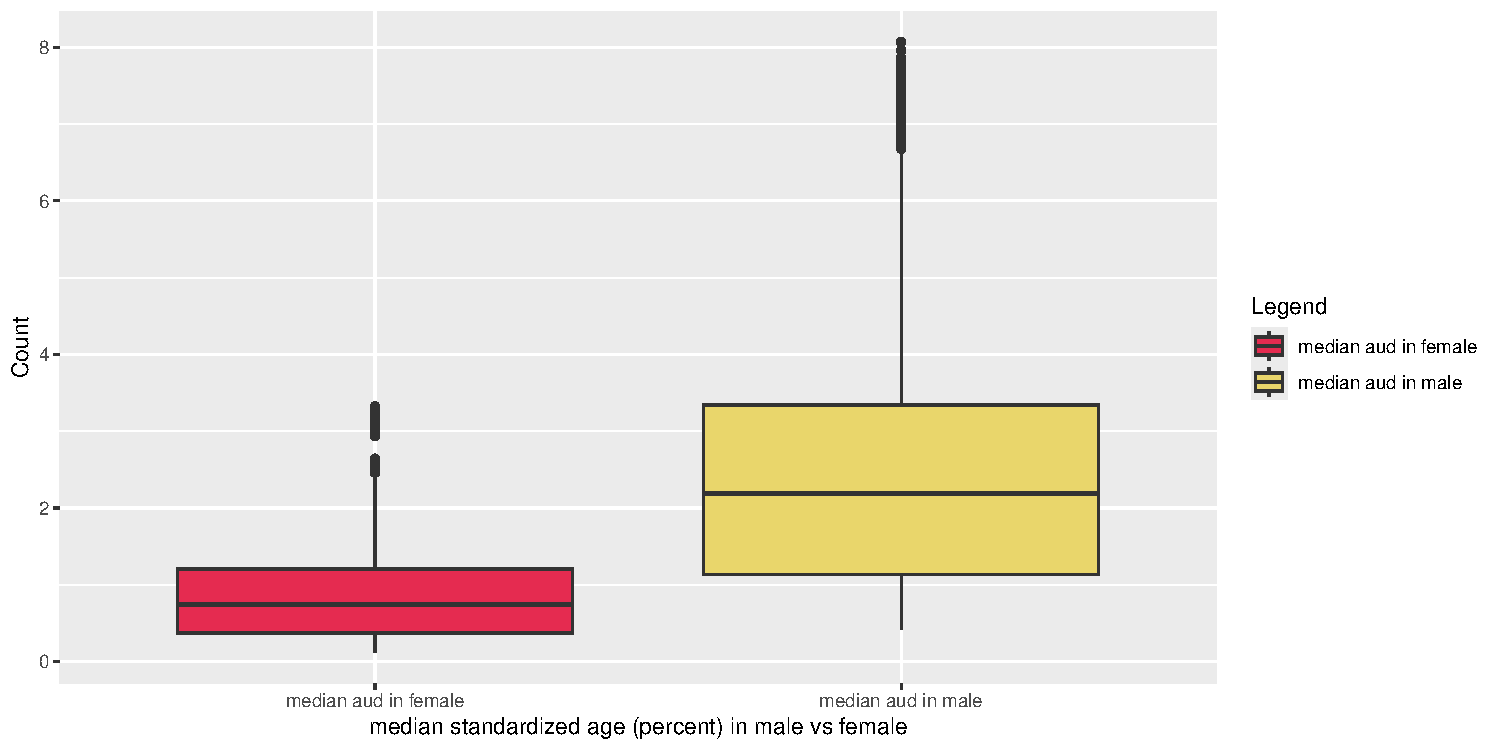
\includegraphics[width=0.7\linewidth]{alcohol_analysis_files/figure-latex/aud1-1} 

}

\caption{Median AUD across standardized age percentage of males and females around the world in 30 years}\label{fig:aud1}
\end{figure}

From the table \ref{tab:alcoholSummary}, it is clear that the mean of Alcohol Use Disorder in male across several years is 2.175 whereas in female it is relatively lower (ie) 0.8416. This table also indicates that the distribution of data is more even in female population around the world over the span of 30 years.

\begin{table}

\caption{\label{tab:alcoholSummary}summary of AUD in male vs female in 2019}
\centering
\begin{tabular}[t]{lll}
\toprule
\begingroup\fontsize{18}{20}\selectfont \cellcolor[HTML]{fae7b5}{\textcolor{black}{ }}\endgroup & \begingroup\fontsize{18}{20}\selectfont \cellcolor[HTML]{fae7b5}{\textcolor{black}{prevalence in female}}\endgroup & \begingroup\fontsize{18}{20}\selectfont \cellcolor[HTML]{fae7b5}{\textcolor{black}{prevalence in male}}\endgroup\\
\midrule
 & Min.   :0.1200 & Min.   :0.420\\
 & 1st Qu.:0.3700 & 1st Qu.:1.140\\
 & Median :0.7150 & Median :2.175\\
 & Mean   :0.8416 & Mean   :2.327\\
 & 3rd Qu.:1.2000 & 3rd Qu.:3.260\\
\addlinespace
 & Max.   :2.9400 & Max.   :7.540\\
\bottomrule
\end{tabular}
\end{table}

\subsection{Alcohol Consumption measure,patterns and trends}\label{alcohol-consumption-measurepatterns-and-trends}

\begin{itemize}
\item
  Alcohol consumption can lead to various detrimental effects .The report aims to explore the standard drinking measures that needs to be taken to avoid the risks that contribute to crimes or accidents.
\item
  The data for this analysis was collected from this \href{https://https://ourworldindata.org/alcohol-consumption\#what-is-a-standard-drink-measure}{website},which provides data on standard drinking measures of different countries.The data was downloaded in CSV format and was imported into R for analysis.
\item
  To analyse the data, tidyverse and ggplot libraries are used for data visualization and exploration.The data has been cleaned and reprocessed to remove the missing values. The variable names have been renamed to make them user-friendly.
\item
  Figure \ref{fig:std-alc} below suggests the standard drinking limits for various countries. It can be clearly understood that the range for standard drinking varies from 0-20 grams per unit. There are countries that have much higher or lower limits.
\end{itemize}

\begin{figure}

{\centering 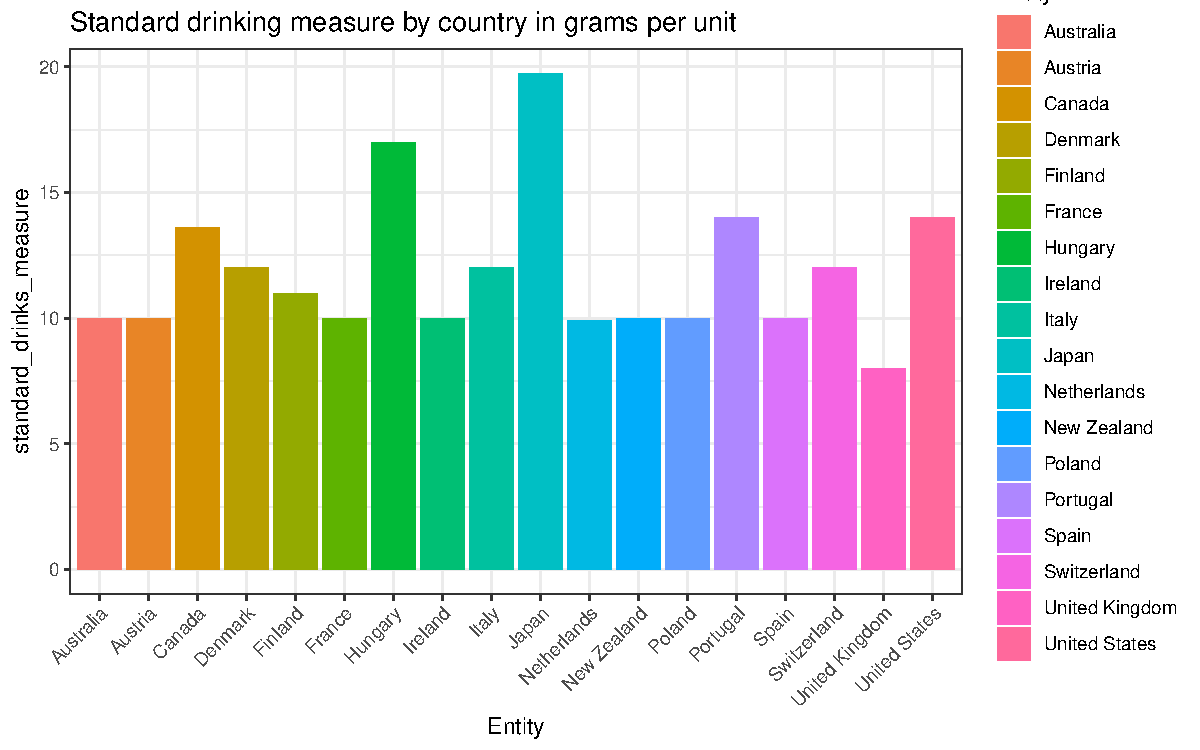
\includegraphics[width=0.7\linewidth]{alcohol_analysis_files/figure-latex/std-alc-1} 

}

\caption{Standard drinking measure by country in grams per unit}\label{fig:std-alc}
\end{figure}

\begin{itemize}
\tightlist
\item
  To gain further understanding, table \ref{tab:table1} presents information on the standard drinking measure for each country by calculating the mean. The mean provides a measure of the variability in the standard drink measure. It is then distributed as low, medium, high and very high based on the amount of alcohol in grams per unit.
\item
  The below table \ref{tab:table1} suggests that some countries have a higher content per serving than others, as it's evident that the Standard Drink Category column is high or very high. This information can be helpful for understanding alcohol consumption trends in order to identify different risks such as road accident deaths associated with alcohol consumption.
  \pagebreak
\end{itemize}

\begin{longtable}[]{@{}llr@{}}
\caption{\label{tab:table1}Mean Standard Drink Categories by Country}\tabularnewline
\toprule\noalign{}
Country & Standard Drink Category & Mean Standard Drink \\
\midrule\noalign{}
\endfirsthead
\toprule\noalign{}
Country & Standard Drink Category & Mean Standard Drink \\
\midrule\noalign{}
\endhead
\bottomrule\noalign{}
\endlastfoot
Australia & Medium & 10.00 \\
Austria & Medium & 10.00 \\
Canada & High & 13.60 \\
Denmark & High & 12.00 \\
Finland & High & 11.00 \\
France & Medium & 10.00 \\
Hungary & Very High & 17.00 \\
Ireland & Medium & 10.00 \\
Italy & High & 12.00 \\
Japan & Very High & 19.75 \\
Netherlands & Medium & 9.90 \\
New Zealand & Medium & 10.00 \\
Poland & Medium & 10.00 \\
Portugal & High & 14.00 \\
Spain & Medium & 10.00 \\
Switzerland & High & 12.00 \\
United Kingdom & Medium & 8.00 \\
United States & High & 14.00 \\
\end{longtable}

\section{Results}\label{results}

\subsection{Global Patterns of Alcohol Consumption}\label{global-patterns-of-alcohol-consumption}

Regardless of the beverage's types, they are all growing in popularity over time, which shows a significant shift in peoples' drinking habits.
For instance, it is observable that in figure \ref{fig:graph} , spirits are highly consumed by Japanese despite being the least popular in other nations.
Additionally, Japan has low consumption in wine and beer, which are the most common in other countries.

\begin{figure}

{\centering 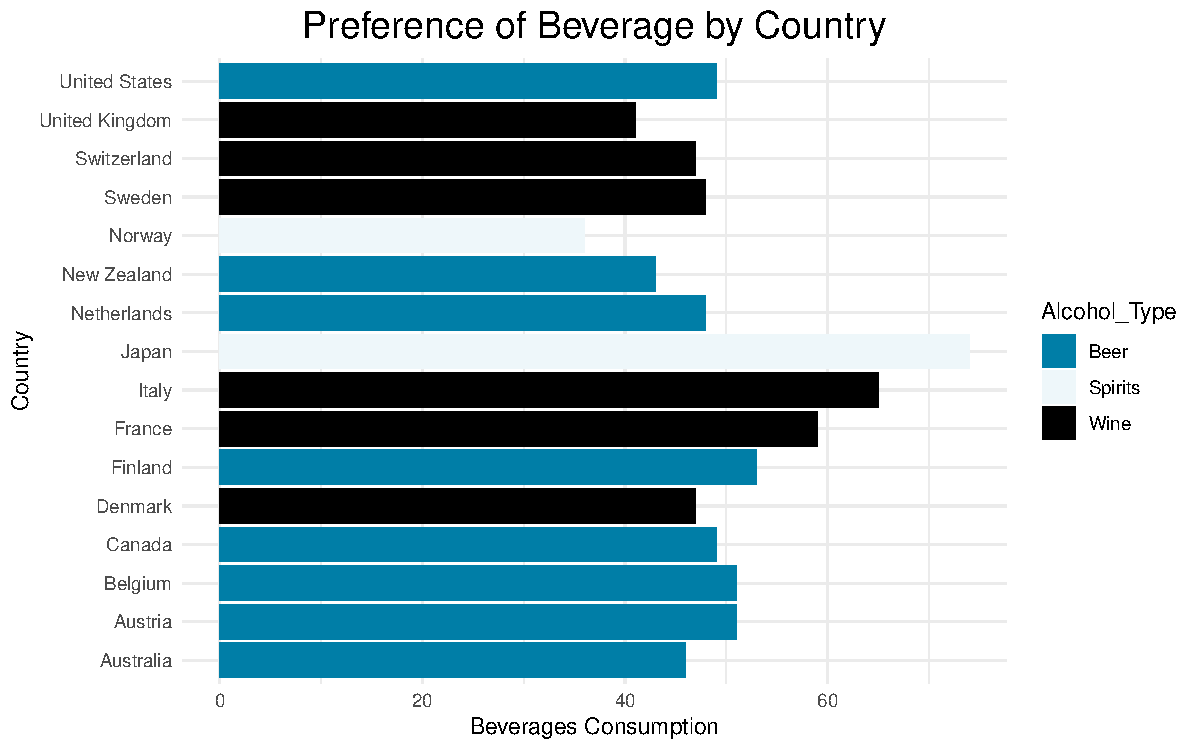
\includegraphics[width=400px,height=250px]{alcohol_analysis_files/figure-latex/graph-1} 

}

\caption{Preference of Beverage by Country}\label{fig:graph}
\end{figure}

Overall, these results emphasize the significance of tracking alcohol consumption patterns
and encouraging responsible drinking behaviors to avoid the unfavorable health and social effects of binge drinking.

\subsection{Global Expenditure on Alcohol}\label{global-expenditure-on-alcohol}

Figure \ref{fig:GDP-vs-Consumption} shows that countries with higher GDP per capita drink more alcohol than those with lower income despite some outliers, indicating a possible linear relationship between the total alcohol consumption per capita and the GDP per capita. Noticeably, European countries' alcohol consumption outweighs that of other continents. However, figure \ref{fig:Population-vs-Consumption} shows random observations not following straight-line patterns, implying that linear relationships might not exist between these variables.
Besides, the Pearson correlation coefficient from the linear regression consumption versus GDP is 0.3835335, indicating a weak positive linear relationship between the total alcohol consumption per capita and the GDP per capita in 2018. Meanwhile, that of consumption versus population model is -0.003349, implying no linear relationship exists. Moreover, the reported \(R^2\) is 0.1470979, showing that 14.71 \% of the variation in the total alcohol consumption per capita can be explained by the variation in the GDP per capita in 2018.
Besides, there are some interesting facts related to the USA - a leading country in GDP, alcohol consumption, and expenditure. By observing its spending on alcohol measured in 2021 inflation-adjusted dollar in figure \ref{fig:US-alcohol-exp}, this amount has increased massively over time, which is mostly spent on alcohol from liquor stores to consume at home.

\begin{figure}

{\centering 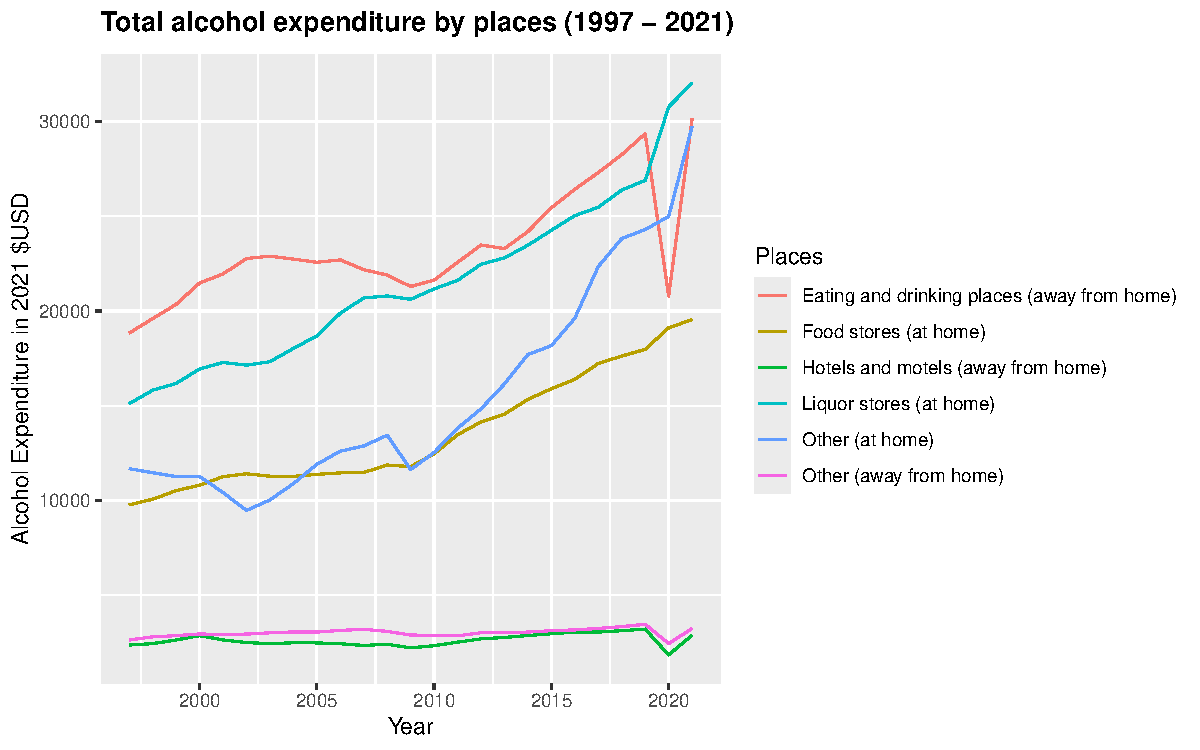
\includegraphics[width=0.7\linewidth]{alcohol_analysis_files/figure-latex/US-alcohol-exp-1} 

}

\caption{Alcohol Expenditure in USA (2000 - 2022)}\label{fig:US-alcohol-exp}
\end{figure}
\pagebreak

\subsection{Current Sitatuation of Alcohol Use Disorder}\label{current-sitatuation-of-alcohol-use-disorder}

The scatter plot (figure \ref{fig:top10} ) compares the prevalence of alcohol use disorders (AUD) in males versus females in 2019 for the top 10 countries with high rates of mental disorders related to alcohol abuse.
After investigating the data for the top 10 countries in terms of total population, it is evident that the percentage of individuals with AUD is significantly higher in males across all leading countries, with Russia, the United States, and Brazil exhibiting particularly higher ratios than the other countries.
Additionally, it is noteworthy that among the top 10 countries, those in Asia, despite having the largest population, have relatively much lower percentage of individuals suffering from the mental health impacts of alcoholism compared to other continents.

\begin{figure}

{\centering 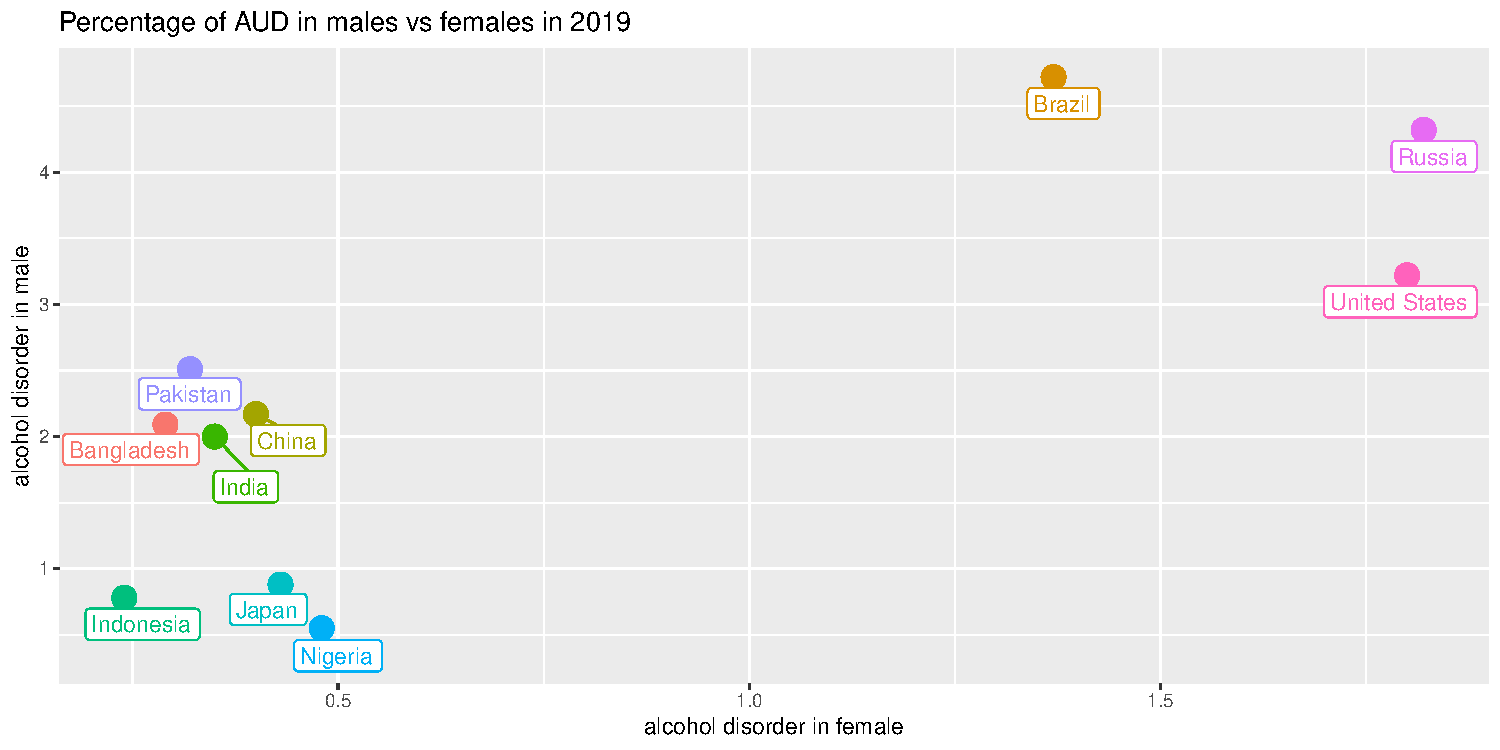
\includegraphics[width=0.7\linewidth]{alcohol_analysis_files/figure-latex/top10-1} 

}

\caption{Percentage of prevalence of AUD in males vs females in 2019}\label{fig:top10}
\end{figure}

\subsection{Road-traffic accident deaths due to Alcohol}\label{road-traffic-accident-deaths-due-to-alcohol}

Based on the results obtained from table \ref{tab:table1},it is understandable that alcohol consumption is a significant problem worldwide which should demand special attention.The below figure \ref{fig:figure2} provides information regarding the top 10 countries with the highest road-traffic deaths associated with alcohol consumption.
It shows that although drivers comply with the standard alcohol drinking measures, an enormous number of road accident deaths still occur.The majority of the countries' figures exceed 50\%, which is an alarming rate.

\begin{figure}

{\centering 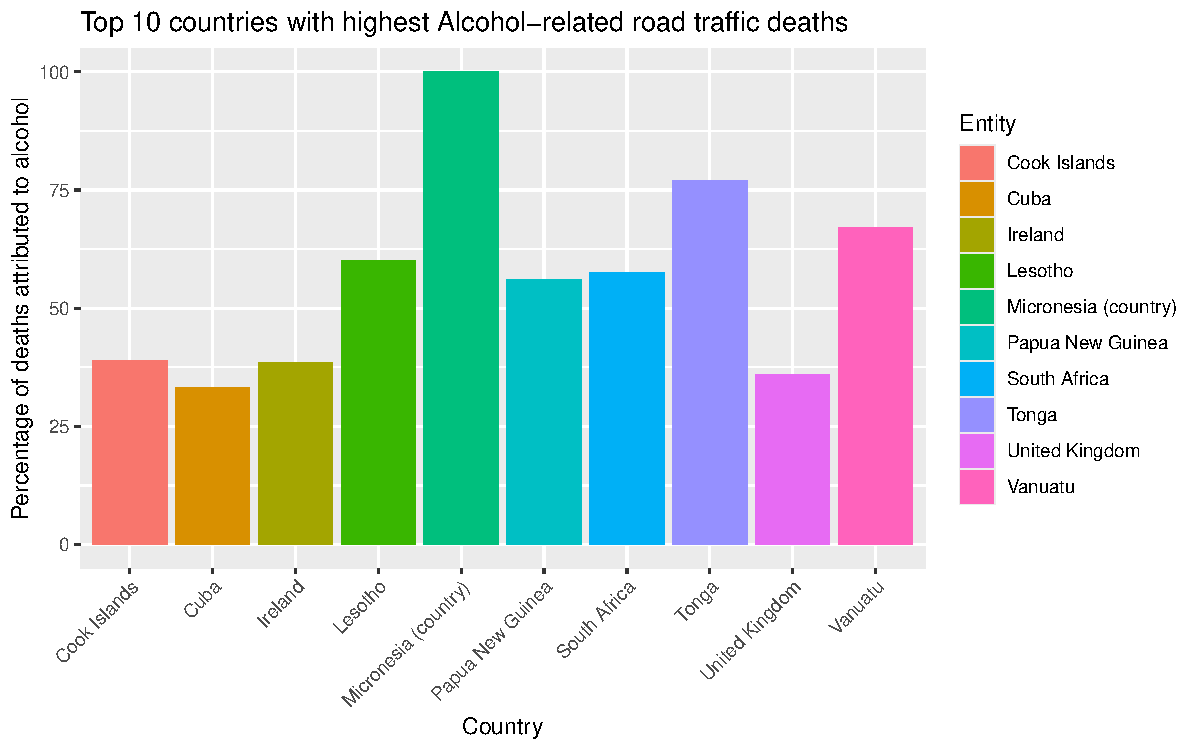
\includegraphics[width=0.7\linewidth]{alcohol_analysis_files/figure-latex/figure2-1} 

}

\caption{Top 10 countries with highest Alcohol-related road traffic deaths}\label{fig:figure2}
\end{figure}

\section{Discussion,Conclusion and Recommendations:}\label{discussionconclusion-and-recommendations}

Based on the analysis of the data sets, multiple inferences regarding the effects of alcohol consumption can be drawn based on four influencing factors, namely, consumption preferences, expenditure, alcohol use disorder, and consumption measures.

Concerning consumer preferences, significant regional differences in the amount of alcohol consumed per person and how people consume beverages were found. From the table \ref{tab:table} it can be concluded that Beer is the most popular beverage, followed by wine and spirits. Secondly, the Middle East and North Africa have very little to no consumption, while Europe has the highest rates.

With respect to alcohol expenditure, there seems to be insufficient evidence to conclude that people from high-income or highly populated countries drink more than others, as both linear models' reported \(R^2\) values are low. However, according to \textcite{owidalcoholconsumption}, many affluent countries consume more copious amounts of alcohol than others, including the USA, as shown in figure \ref{fig:US-alcohol-exp}.

The pattern of the alcohol use disorder is presented in figure \ref{fig:top10}, demonstrating a more significant percentage of males being affected by the prevalence of alcohol use disorders due to alcoholism than that of females across the top 10 most populous countries worldwide. Moreover, despite having the largest population, Asian countries have fewer people suffering from AUD and its related mental health impacts of alcoholism than other continents.

In the case of alcohol consumption measures and road-traffic deaths, it can be concluded from figure \ref{fig:std-alc} and figure \ref{fig:figure2} that, even after having standard alcohol drinking measures, alcohol consumption is still a concern as due to an inordinate number of deaths in road traffic accidents.

Based on our conclusion, it is recommended that countries should prioritize running interventions and aid groups as a method to alleviate the situation of alcohol-related disorders and provide help for the victims of alcohol abuse. Campaigns on alcohol consumption should be launched to raise awareness about the delimits of alcohol consumption. Policymakers can introduce policies like increasing taxes on alcohol and enforcing strict drunk driving laws. Governments, health organizations, and educational institutions work together to resolve the problem of excessive alcohol consumption and promote responsible drinking habits.

\printbibliography

\end{document}
